\section{缓冲区缓存总体设计}

文件系统并不直接驱动磁盘。普通文件读写、超级块装载、inode 写回和交换区访问都先进入缓冲区缓存，再由缓冲区缓存把块请求交给具体设备。这个中间层保存最近访问过的磁盘块，维护空闲缓冲区队列，处理同步写、延迟写和异步写，并在 I/O 完成后唤醒等待进程。对 Unix V6++ 这类教学系统而言，缓冲区缓存是理解“文件系统为什么不直接面对硬件”的关键模块。

main 分支采用双向链表、状态标志和显式睡眠唤醒维护缓冲区。一个缓冲区在不同时刻可能属于设备缓存链、空闲队列或设备 I/O 请求队列；如果忙标志、延迟写标志和链表挂接顺序不一致，错误往往要到后续 getblk、brelse 或中断完成阶段才暴露。Rust 重构没有改变经典缓冲区缓存算法，而是把状态位、队列链接和数据访问收进较固定的对象接口中。

设备管理本身不是本文展开的重点，保留到本章的原因在于文件系统必须通过块设备接口完成读写。原 C++ 代码中，缓冲区对象、设备请求队列和 ATA/DMA 驱动共享较多底层状态；Rust 版本把“提交块请求”“启动设备传输”“处理中断完成”分成较固定的接口步骤，使后续把 IA32 ATA 路径替换为 RISC-V VirtIO 路径时，不必改写 inode 读写和目录解析逻辑。

Rust 版本继续区分块设备和字符设备，但本章只关注块设备对文件系统的支撑。具体改动包括重新用 Buf、Buffer 和 BufferSlot 描述缓冲区元数据和数据区，通过 BufferManager 与 BlockDevice 接口串联设备请求队列和中断完成路径，并用 trait 约束具体驱动需要实现的 open、close、strategy 和 start 等接口。

\begin{table}[htbp]
  \centering
  \caption{缓冲区与设备管理子模块功能说明表}\label{tab:buffer-device-modules}
  \begin{tabular}{p{0.30\textwidth}p{0.60\textwidth}}
    \toprule
    \textbf{代表文件} & \textbf{主要功能} \\
    \midrule
    dev/buffer.rs & 定义缓冲区缓存相关的基础数据结构，包括 Buf、Buffer、BufRef、BufferData 和 BufferSlot，并提供缓冲区数据访问接口 \\
    dev/buffer\_manager.rs & 实现缓冲区缓存管理逻辑，负责缓冲区获取、释放、预读、延迟写、异步写、交换区 I/O 以及睡眠唤醒协作 \\
    dev/block\_device.rs & 定义块设备抽象接口和设备控制表，实现块设备请求排队、启动和设备队列管理 \\
    dev/ata\_driver.rs & 实现 ATA DMA 驱动，负责设置控制器寄存器、构造 PRD 表、启动 DMA 传输和处理中断完成逻辑 \\
    \bottomrule
  \end{tabular}
\end{table}

\section{缓冲区缓存机制重构}

Rust 版本把缓冲区拆成几类对象。Buf 保存设备号、物理块号、状态标志、剩余字节数、错误码和链表链接；BufferData 保存 512 字节数据区；BufferSlot 在初始化时把一个 Buf 与一块 BufferData 绑定；BufRef 表示对 Buf 的内部引用；Buffer 则是上层读写数据时拿到的包装对象。这样拆分后，状态管理和数据访问不会都挤在同一个裸结构体指针上。

Buf 负责“这块缓存现在属于哪个设备块、处于什么状态、挂在哪个队列上”，BufferData 负责“512 字节内容是什么”。上层通过 Buffer 访问数据，而不是直接拿到任意内存地址。该设计没有改变固定大小缓冲区池的前提，但减少了元数据和数据区被混用的机会。

\begin{figure}[htbp]
  \centering
  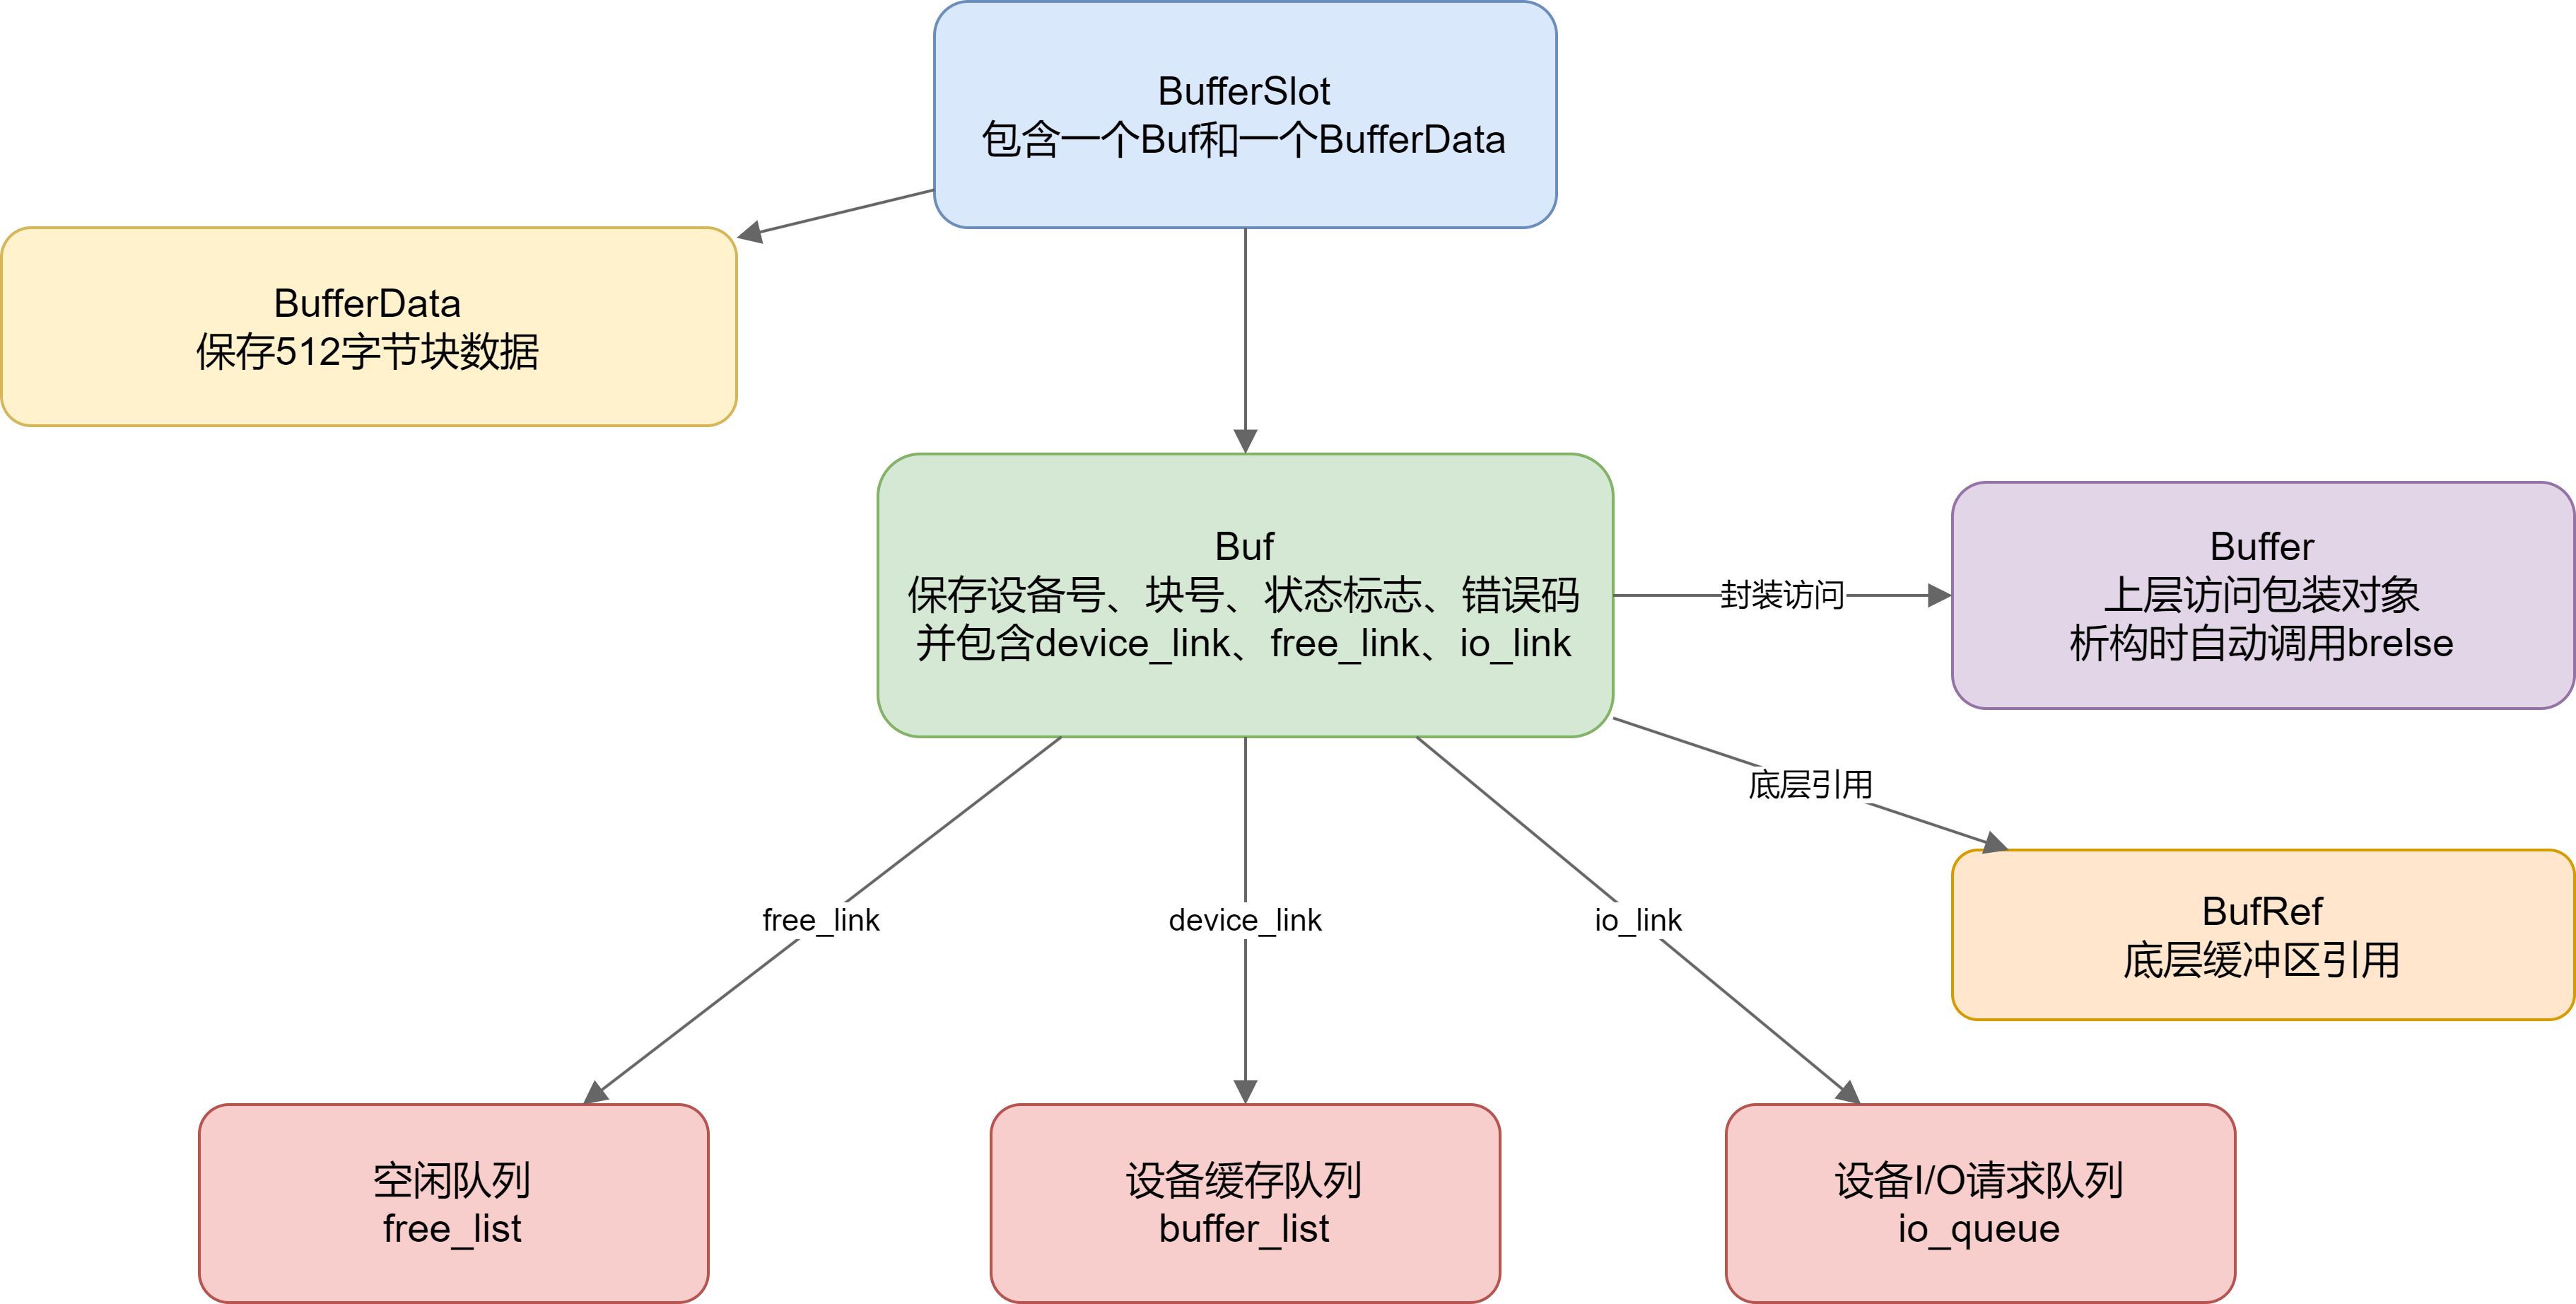
\includegraphics[width=0.72\textwidth]{figures/5/1数据结构.png}
  \caption{缓冲区数据结构与队列关系图}
\end{figure}

BufferManager::get\_blk 和 get\_blk\_ref 负责查找或分配缓冲区。函数先在设备缓存链中查找目标块；命中且未忙时直接返回；命中但忙时，当前进程在该缓冲区等待；未命中时，从空闲队列取出一个缓冲区重新绑定到目标设备块。若选中的缓冲区带有延迟写标志，则先发起异步写回，再重新尝试分配。这一流程保留 Unix 缓冲区缓存的原始思想，代码层面则由 BufferManager 统一维护队列关系。

释放由 brelse 完成。该函数清除忙标志和等待标志，把缓冲区插回空闲队列，并唤醒等待该缓冲区或等待空闲缓冲区的进程。Rust 版本的关键变化在于，外部代码通常不直接改写链表前驱后继，也不直接组合多个标志位；这些操作集中在 BufferManager 内部完成。

队列仍分为空闲队列、设备缓存队列和设备 I/O 请求队列。空闲队列回答“当前哪些缓冲区可重新分配”，设备缓存队列回答“某设备块是否已经在缓存中”，I/O 请求队列则记录已经交给块设备、但尚未完成传输的请求。三类队列对应三种不同问题，不能简单合并。

每个 Buf 同时包含设备链、空闲链和 I/O 链三组链接字段。侵入式链表保留了传统内核链表不额外分配节点的特点，但通过适配器统一插入、删除和遍历接口。对缓冲区缓存而言，这种实现比外部分配链表节点更贴近原算法，也比散落的裸指针操作更容易检查。

预读、延迟写和异步写仍被保留。breada 在顺序访问时读取当前块，并尝试提前提交下一块；bdwrite 只把缓冲区标记为延迟写，不立即等待磁盘完成；bawrite 则提交写请求后释放当前执行流。三者都是传统 Unix 块 I/O 路径中的小型优化，重构时保留它们有助于维持原系统行为。

\section{同步、中断与文件系统协同}

缓冲区缓存仍使用睡眠与唤醒协调进程和设备。目标缓冲区被占用时，进程睡在该缓冲区的等待通道；空闲队列为空时，进程睡在空闲队列相关通道；同步 I/O 发起后，进程等待对应缓冲区完成。这里保留阻塞式模型，是为了与 Unix V6++ 原有调度和 I/O 语义保持一致。

I/O 完成后，io\_done 更新缓冲区状态并唤醒等待者；随后 brelse 可能把缓冲区重新放回空闲队列。这样，设备中断、缓冲区状态和进程调度之间通过等待通道衔接，而不是让上层文件系统忙轮询设备状态。

文件系统与缓冲区缓存的接口集中在 global\_buffer\_manager() 及其 bread、bdwrite、bawrite、bwrite 等方法。inode 读写通过这些方法访问数据块，超级块装载和写回通过缓冲区完成扇区级访问，交换区路径则使用专门的 swap 接口。文件系统层因此不必知道当前块最终由 ATA、VirtIO 还是其他设备完成传输。

这一点对 RISC-V 迁移很重要。第 5 章中块设备从 ATA 切换到 VirtIO 后，文件系统上层仍沿用 bread 和 bdwrite 等接口；需要替换的是块设备实现，而不是 inode 读写和目录解析算法。

\section{块设备驱动重构}

refactor/x86 分支的块设备仍基于 ATA 控制器和 DMA。ATADriver 设置 ATA 寄存器，构造 DMA PRD 表，启动总线主控 DMA 传输，并在磁盘中断到来后检查状态、结束请求。LBA28 寻址、ATA 命令字和 DMA 控制寄存器仍沿用原系统做法，因此这一章讨论的是 Rust 表达方式的重构，而不是 IA32 块设备模型的替换。

发起请求时，驱动从缓冲区取得设备号、物理块号和传输长度，填写 ATA 控制寄存器与 DMA PRD 表。读请求和写请求分别对应不同 ATA DMA 命令，完成后再由中断处理函数把结果反馈给缓冲区管理器。

一次块请求的路径大致如下。文件系统或交换区调用缓冲区接口后，BufferManager 取得目标缓冲区，并调用块设备的 strategy；块设备把缓冲区插入设备 I/O 队列；设备空闲时，start 取出队首请求并调用 ATADriver::dev\_start；磁盘中断到来后，ATADriver::ata\_handler 检查错误状态、更新设备活动标志、弹出已完成请求，并通知 BufferManager 执行 io\_done；等待该缓冲区的进程随后被唤醒。

这条路径把职责分成三层。缓冲区缓存层管理块对象和等待关系，块设备层管理请求队列，驱动层处理寄存器和 DMA。后续替换底层驱动时，最理想的情况是只替换第三层和少量设备注册逻辑。

\begin{figure}[htbp]
  \centering
  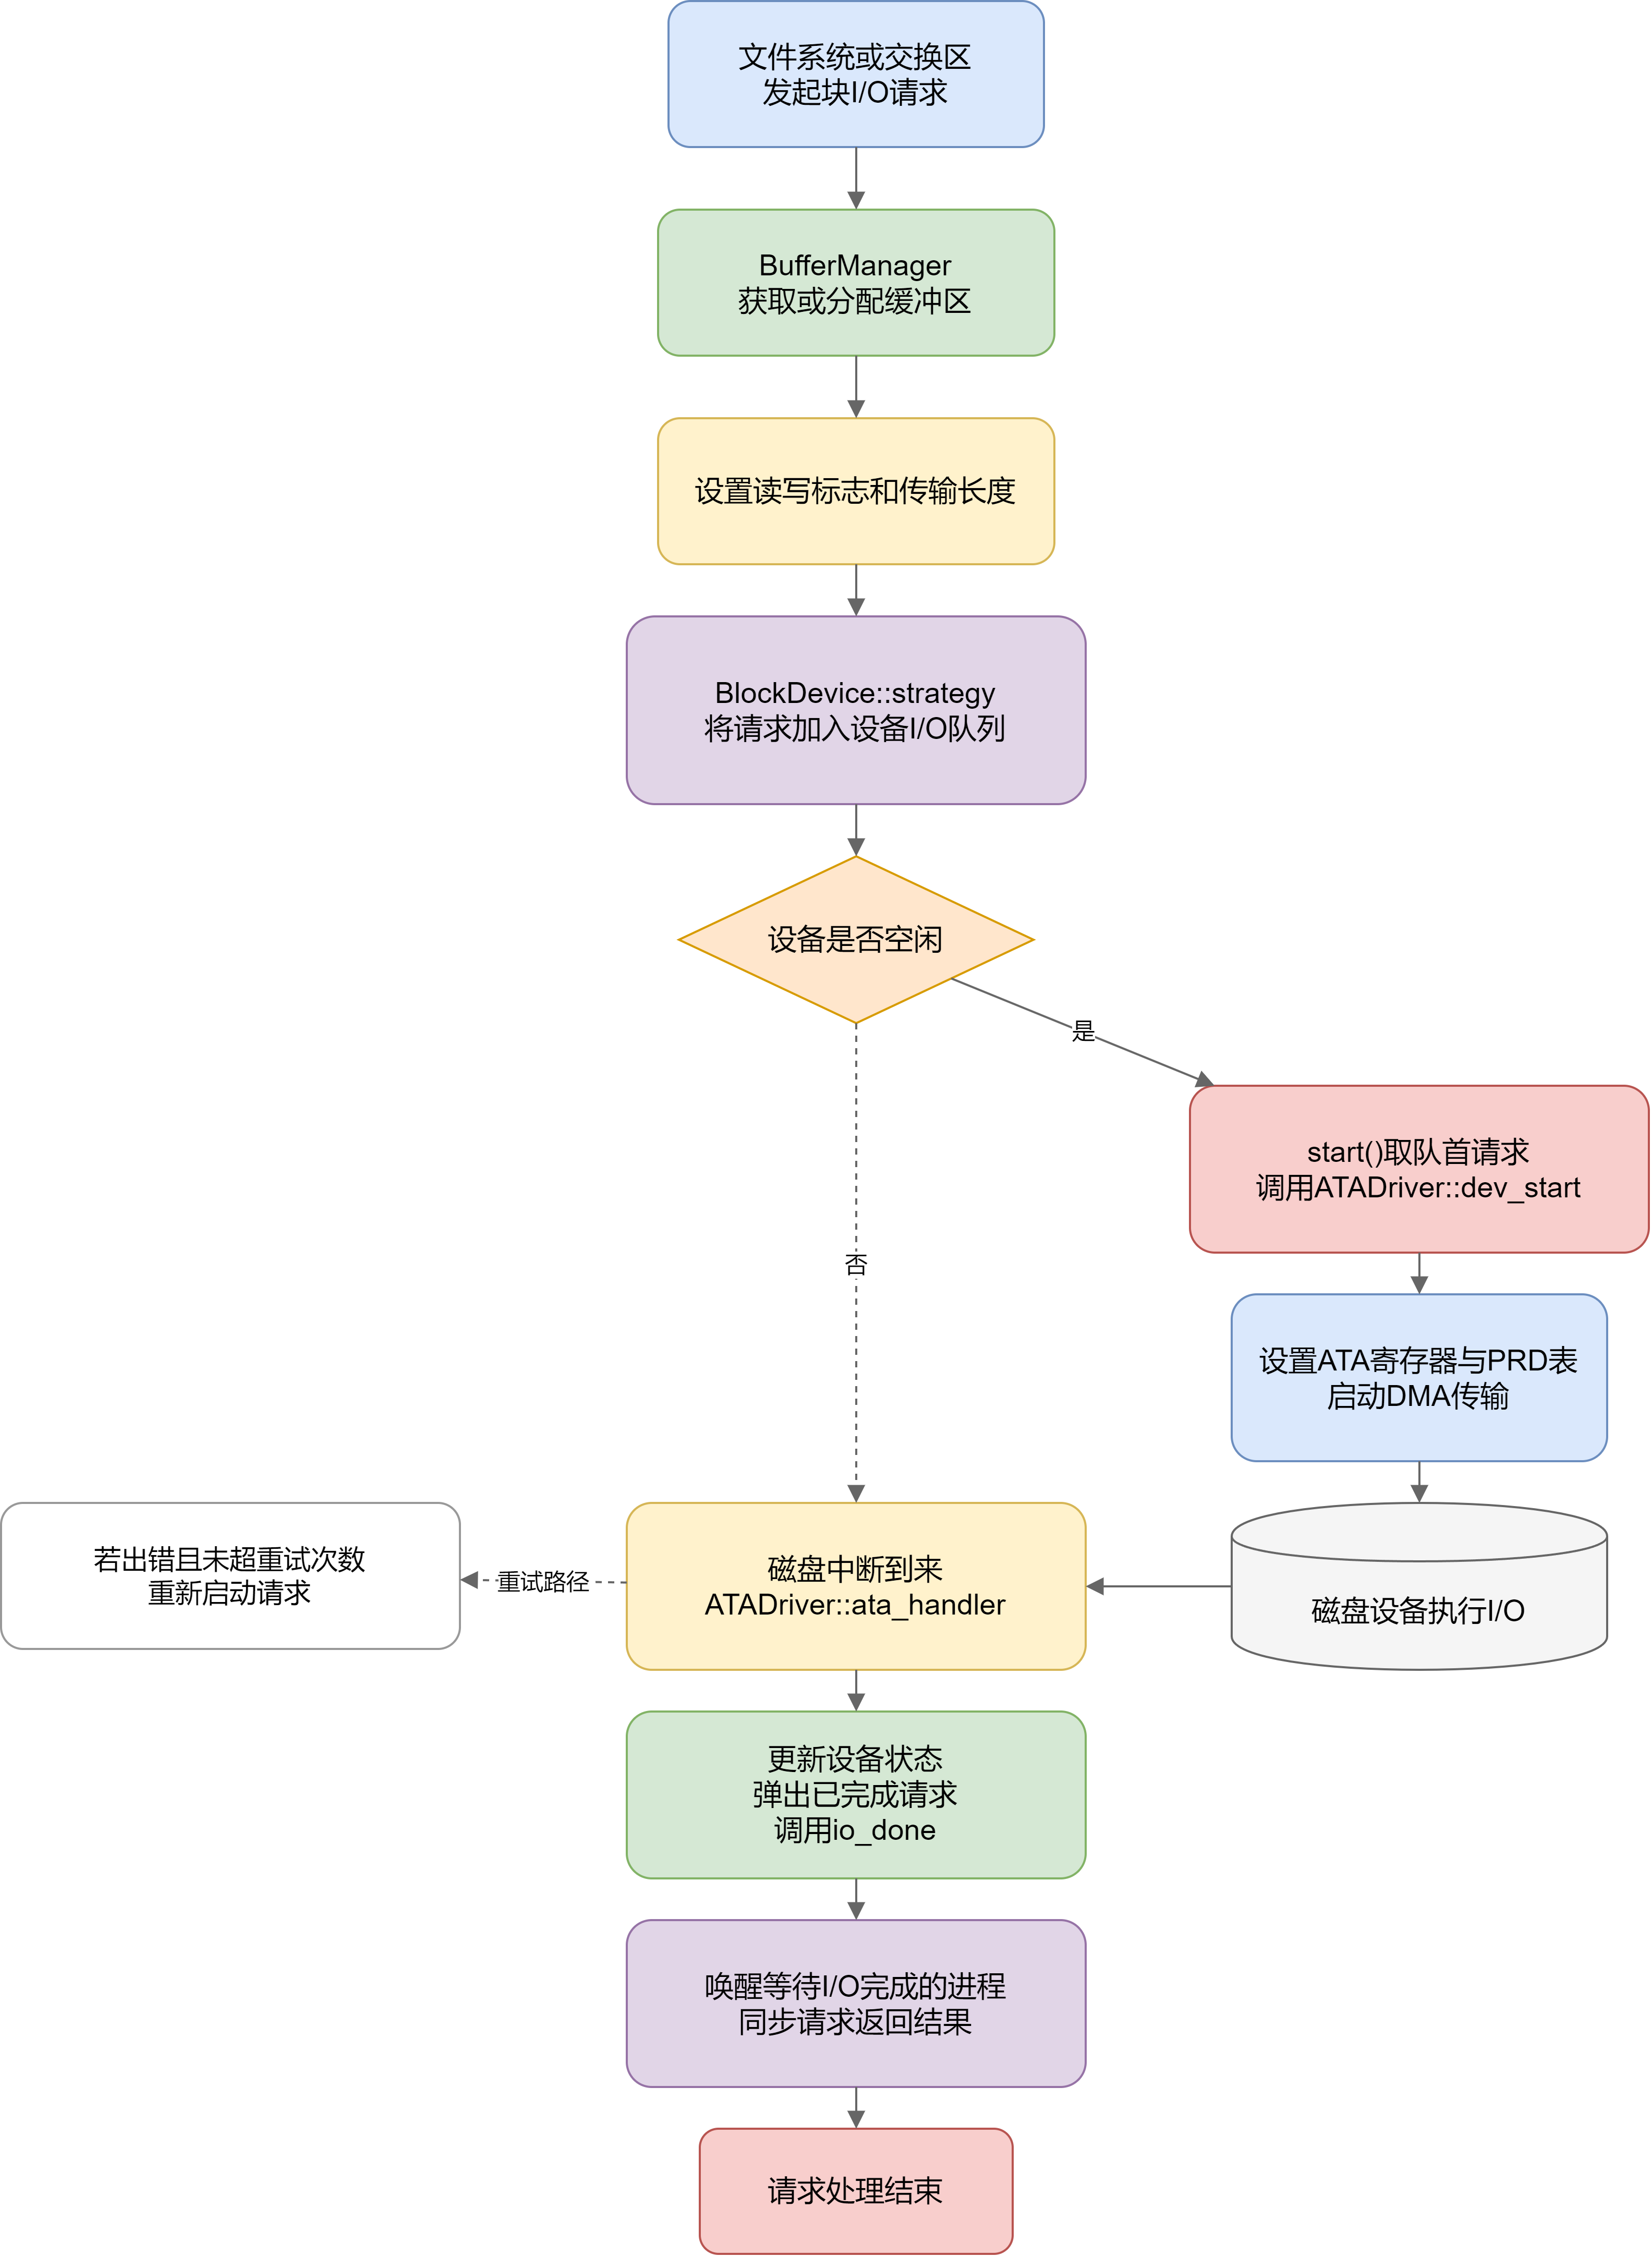
\includegraphics[height=0.62\textheight,keepaspectratio]{figures/5/2块设备.png}
  \caption{块设备请求处理流程图}
\end{figure}

BlockDevice trait 描述块设备需要提供的 open、close、strategy、start 和 devtab 等接口。当前 IA32 分支中，块设备主要由 ATABlockDevice 实现；RISC-V 分支则由 VirtIO 块设备实现同类接口。这样处理后，设备分发仍然存在，但文件系统看到的是固定块设备接口，而不是某个具体控制器的寄存器操作。

\section{本章小结}

本章围绕文件系统与缓冲区缓存的 Rust 重构展开。磁盘格式、目录项结构和多级块索引保持 Unix V6++ 原有逻辑，重构重点放在内存表示、引用关系、错误路径和块 I/O 边界上。InodeRef、FileRef、InodeRefGuard、Result 和 PosixError 共同承担了原先由裸指针、全局状态和调用约定维持的部分责任。缓冲区路径中，Buf、Buffer、BufferSlot、BufferManager 和 BlockDevice 等对象重新组织了缓存状态、队列挂接、睡眠唤醒和设备请求完成过程。经过这些调整，文件系统仍能呈现原有教学机制，同时更便于检查 inode、文件对象和缓冲区之间的资源关系。
